\documentclass[aps, prl, reprint, showpacs]{revtex4-1}
\pdfoutput=1

\usepackage{booktabs}
\usepackage{graphicx}
\usepackage{multirow}
\usepackage{subfigure}
\usepackage[hyperindex,breaklinks,hidelinks,colorlinks,allcolors=blue]{hyperref} 

\begin{document}

\title{Classifying Party Affiliation Based on Campaign Rhetoric}

\author{Rory Fitzpatrick (\textit{roryfitz}), Garrett Merz (\textit{gwmerz}), Julia Pakela (\textit{jpakela})}
%\collaboration{ATLAS Collaboration}

\begin{abstract}
\noindent Machine learning has been vastly applied to natural language processing. We report the performance of several classification methods used to determine political party based on campaign rhetoric. We use corpora of campaign speeches from the 1960, 2008 and 2016 election cycles. Finally, we investigate the use of classification performance as a metric for quantifying party polarization as a function of time.
\end{abstract}

%\pacs{13.38.Dg}

\maketitle

%%% INTRODUCTION %%%
\section{Introduction}
In the era of the 24/7 news cycle, political rhetoric has transformed into the stringing-together of sound bites to be swept up by the media and repeated out of context \textit{ad infinitum}. Political speech is rife with partisan buzzwords, a rhetorical structure that may lend itself to classifying party affiliation based on political discourse. In addition to providing a unique classification scheme, party affiliation classifiers could provide a metric for quantifying political polarization in a given election cycle or administration. We show that we can accurately classify political campaign speech based on the party of the speaker, and in turn use the classification performance over time to quantify party polarization. 

%%% DATA %%%
\section{Datasets and Data Processing}
We use bipartisan campaign rhetoric curated in \cite{peters} from the 1960, 2008, and 2016 election cycles. We selected these years because they each contained a large sample of speech from both political parties and occur at dramatically different points in the country's political history. We excluded, for instance, the 2012 election cycle, because the speeches collected from the Obama campaign are all variations of the same stump speech, and would bias the classifier. Initially, words contained in the  Python \texttt{nltk} `stopwords' and `names' corpora are removed from each document. We acknowledge that there are still many names and proper nouns that are included in our resulting vocabularies. Further study could be done on the effect of removing or keeping all proper nouns (e.g. one might expect ``Reagan" to be more common in Republican speeches) but it is outside the scope of this report.

We lemmatize and stem using the \texttt{nltk} \texttt{WordNetLemmatizer} and \texttt{PorterStemmer} to reduce variations in words. No effort is made to correct typos. The resulting texts are converted to the bag-of-words format using three different frequency measures: \textbf{(1)} standard term frequency (\textit{tf}), \textbf{(2)} presence or absence of a word (\textit{bool}) and \textbf{(3)} a frequency measure known as term frequency-inverse document frequency (\textit{tfidf}). The \textit{tfidf} frequency is calculated as follows:
\begin{equation}
    w = f_{t,d} \ln (1 + N/n_t),
\end{equation}
where $f_{t,d}$ is the frequency of the word in the current speech, $N$ is the total number of documents in the training set, and $n_t$ is the number of documents in the training set that contain the word. We have also chosen to add one to the argument of the log for smoothing. We do not restrict the size of the bag-of-words vocabulary. Further study could be done to determine whether a restricted vocabulary (e.g. the 5000 most common training words) improves or worsens classification ability.

\begin{table}[h] % use table* for two-column table
  \label{tab:data}
  \begin{ruledtabular}
  %  \newcommand{\twrw}[1]{\multirow{2}{*}{#1}}
  \begin{tabular}{cccc}
   & 1960 & 2008 & 2016 \\
 \hline
    Democrat & 598 & 362  & 76  \\
    Republican & 311 & 222  & 82  \\

 \hline
  \end{tabular}
  \end{ruledtabular}
    \caption{The number of speeches available for each election cycle.}
\end{table}

%%% METHODS %%%
\section{Classification Methods}
Similar studies have been done using floor speech from the Senate and House of Representatives in \cite{yu} which uses the popular text classification methods, Naive Bayes (NB) and Support Vector Machines (SVM) However, it was shown in \cite{kwon} and \cite{thomas} that these methods are sensitive to outliers. We speculate that this is why in \cite{yu} it was found that House speeches were better suited than Senate speeches for training party classifiers - the House is considered to be more partisan than the Senate, and documents from this group would presumably contain fewer outlier events. In addition to the naive methods for classification, we implement robust methods for SVM  as described in \cite{chandra} and \cite{xu} to investigate whether it is possible to design a classifier which is better suited for training on texts from more moderate speakers. We also test classification methods less traditionally used for text classification: logistic regression (LR) and $k$-nearest neighbors (KNN). We begin by training an cross-validating within a single election cycle for each classification method and each word frequency measure.  Then, we train on a single election cycle and test on the remaining two election cycles. We also report, based on the NB method, the words most indicative and Democratic and Republican speech in each election cycle and across all three cycles.

\subsection{Robust SVMs}
The classification methods described above have limited sensitivity to outliers. You could imagine that a political party ``outlier" could exist if a candidate was associated with a particular party but came into an election intending to focus on topics that have yet to gain prominence as a debate topic during campaigns. We attempt to improve upon the classification methods above by implementing a robust method of SVM like the one described in \cite{xu}. Here we will detail the minimization problem.


%%% RESULTS %%%
\section{Results}

We use both cross validation and traditional training/testing to gain insights into partisanship in US campaigns for the 1960, 2008 and 2016 election cycles. We use cross validation within single election cycles to optimize model parameters (e.g. $C$ in SVM or $k$ in KNN). Comparing the cross validation scores between election cycles can give some insight into degree of polarization between parties; if parties are highly polarized, cross validation scores should be greater. We then train with data from one election cycle and test on the remaining two. This can quantify the degree to which party lines shift between election cycles. The results for each set of tests are summarized below.

\subsection{Cross validation}

Results shown in Table \ref{tab:crossval}.

We find that the boolean word frequency measure does best in cross validation tests for NB, SVM and LR.

\subsection{Predictions between years}

We expect party values and talking points to evolve over time, we expect at least some predictive power when training on data from one election cycle and testing on another. Classification tends to do better when trained and tested on election cycles that are closer temporally. This is expected; the topics of interest change less between consecutive cycles than over the course of several decades. This is evident from the results in Table \ref{tab:results}. 2008 and 2016 are far better at predicting party affiliation in speeches between the two cycles than either is at predicting party affiliation in the 1960 election. In fact, when training on 1960 and testing on 2008/2016 and vice versa, we often to do worse than randomly guessing. This is reasonably consistent across classification schemes and word frequency metrics. We find that the most common misclassifications are 1960s Republicans being labeled as Democrat when trained with 2008 and 2016 data.

\subsection{Predictive words}

The most predictive words for each party for each election cycle (and for all three combined) are shown in Table \ref{tab:words}. Particularly for the \textit{tf} and \textit{bool} frequency measures, the most common words strike a chord as the common sticking point for a particular election cycle. Though not listed, the fourth most indicative word for Democratic speech in 1960 was ``catholic"; Kennedy was the first Catholic president. Kennedy was also in the habit of listing prominent Republicans from the last century during his speeches, hence the indicative power of ``coolidg" (Calvin Coolidge, 30th President) and ``landon" (Alf Landon, 1936 Republican nominee). In 2008, race, of course, was a prominent topic, but so was economic strategy; ``trickle" (as in ``trickle-down economics," coined during the Reagan era) was a common word used by the Democrats to oppose large tax cuts to the wealthy. McCain commonly used the phrase ``shoulder a rifle" when expressing support for the troops --- he was a well-known war veteran himself. In 2016 multiple top words refer to wealth (``billionaire" and ``millionaire") and equality (``fairer" and ``ineq," the stem of words like ``inequality"). There's an indirect reference to Clinton's emails (``delet" --- this was a common talking point for Trump). And healthcare made the top contenders in 2016 as well: ``obamacar" was indicative of Republican speech (it was yet another common talking point for Trump). These words provide a unique lens into the politics of the era and are interesting in their own right. We see signs of the most prominent social, economic, and political issues during each election period.

\begin{table} % use table* for two-column table
  \begin{ruledtabular}
  %  \newcommand{\twrw}[1]{\multirow{2}{*}{#1}}
  \begin{tabular}{ccccc}
  Method & Freq.& 1960 & 2008 & 2016 \\
    \hline
 & \textit{tf} & 92.0  & 81.1 & 91.7 \\
NB & \textit{bool} & 92.7  & 83.0 & 92.9 \\
 & \textit{tfidf} & 91.1  & 83.9 & 93.0 \\
 \hline
 & \textit{tf} & 91.4 & 87.1 & 85.6 \\
SVM & \textit{bool} & 93.3 & 91.2 & 91.2 \\
 & \textit{tfidf} & 91.8 & 86.0 & 90.5 \\
 \hline
   & \textit{tf} & 89.8  & 88.2 & 85.6 \\
LR & \textit{bool} & 93.3  & 92.9 & 91.2 \\
 & \textit{tfidf} & 90.1  & 88.3 & 89.3 \\
 \hline
   & \textit{tf} & ZZ  & ZZ & ZZ \\
KNN & \textit{bool} & ZZ  & ZZ & ZZ \\
 & \textit{tfidf} & ZZ  & ZZ & ZZ \\
 \hline
  & \textit{tf} & ZZ  & ZZ & ZZ \\
RSVM & \textit{bool} & ZZ  & ZZ & ZZ \\
 & \textit{tfidf} & ZZ  & ZZ & ZZ \\
 \hline
  \end{tabular}
  \end{ruledtabular}
    \caption{Cross validation scores by method and word frequency metric.}
     \label{tab:crossval}
\end{table}

\begin{table*} % use table* for two-column table
  \begin{ruledtabular}
  %  \newcommand{\twrw}[1]{\multirow{2}{*}{#1}}
  \begin{tabular}{ccccc}
   Method & Training Year & 1960 (\textit{tf}/\textit{bool}/\textit{tfidf}) & 2008 (\textit{tf}/\textit{bool}/\textit{tfidf}) & 2016 (\textit{tf}/\textit{bool}/\textit{tfidf}) \\
    \hline
 & 1960 & ---  & \textit{41.8}/\textit{43.2}/46.2 & 46.5/53.5/48.4 \\
NB & 2008 & \textit{43.6}/54.1/48.2  & --- & 58.6/54.8/\textbf{63.1} \\
 & 2016 & \textbf{63.4}/\textbf{64.0}/\textbf{64.1}  & \textbf{63.5}/\textbf{63.2}/\textbf{63.4} & --- \\
 \hline
  & 1960 & ---  & \textit{42.8}/51.9/\textit{43.3} & 54.8/47.8/48.4 \\
SVM & 2008 & \textit{42.2}/48.0/46.8  & --- & 58.6/54.8/48.4 \\
 & 2016 & \textit{40.4}/53.5/49.5  & \textbf{66.1}/\textbf{66.8}/\textbf{70.0} & --- \\
 \hline
  & 1960 & ---  & 47.1/51.0/48.3 & 54.1/47.1/55.4 \\
LR & 2008 & \textit{41.3}/47.1/\textit{44.4}  & --- & \textbf{66.2}/59.2/50.3 \\
 & 2016 & 51.8/55.9/51.5  & \textbf{67.1}/\textbf{67.8}/\textbf{71.2} & --- \\
 \hline
  & 1960 & ---  & ZZ/ZZ/ZZ & ZZ/ZZ/ZZ \\
KNN & 2008 & ZZ/ZZ/ZZ  & --- & ZZ/ZZ/ZZ \\
 & 2016 & ZZ/ZZ/ZZ  & ZZ/ZZ/ZZ & --- \\
 \hline
  & 1960 & ---  & ZZ/ZZ/ZZ & ZZ/ZZ/ZZ \\
RSVM & 2008 & ZZ/ZZ/ZZ  & --- & ZZ/ZZ/ZZ \\
 & 2016 & ZZ/ZZ/ZZ  & ZZ/ZZ/ZZ & --- \\
 \hline
  \end{tabular}
  \end{ruledtabular}
    \caption{CAPTION results for training on one year and testing on another \textbf{bold} $> 60\%$, \textit{italics} $< 45\%$.}
     \label{tab:results}
\end{table*}

\begin{table*} % use table* for two-column table
  \begin{ruledtabular}
  %  \newcommand{\twrw}[1]{\multirow{2}{*}{#1}}
  \begin{tabular}{cccc}
  Year & Freq. & Democrat & Republican \\
    \hline
 & \textit{tf} & coolidg, landon, forsight  & incident, standpoint, surrend   \\
1960 & \textit{bool} & coolidg, landon, forsight   & incident, standpoint, tear  \\
 & \textit{tfidf} & dribble, cold, blackwel  & hanov, corrobor, conced  \\
 \hline
 & \textit{tf} & dime, trickl, racial  & brokaw, constru, jihadist  \\
2008 & \textit{bool} & dime, trickl, workplac  & rifl, despis, discretionari  \\
 & \textit{tfidf} & bricklay, highli, jindal  & assuage, dispatch, best  \\
 \hline
 & \textit{tf} & billionair, wealthiest, vermont  & obamacar, renegoti, delet   \\
2016 & \textit{bool} & billionair, fairer, ineq   & delet, renegoti, salut    \\
 & \textit{tfidf} & bad, quito, protest    & machin, outlcass, conspicu   \\
 \hline
  & \textit{tf} & billionare, coolidg, landon   & standpoint, obamacar, incident  \\
combined & \textit{bool} & coolidg, billionare, landon   & standpoint, delet, incident  \\
 & \textit{tfidf} & alumnu, avert, compulsori  & animos, downplay, barren  \\
 \hline
  \end{tabular}
  \end{ruledtabular}
    \caption{The words most indicative of both political parties based on election year and word frequency metric.}
    \label{tab:words}
\end{table*}


%%% CONCLUSIONS %%%
\section{Conclusions}

Further study could be done to expand the dataset to examine the change of rhetoric from year to year and explore how long a particular election cycle might be predictive for future election cycles.

Another confounding factor may be the presence or absence of an incumbent running in the election for a particular year. This candidate would have no opponent within their own party and may speak differently as a result.

%\begin{figure}[h]
%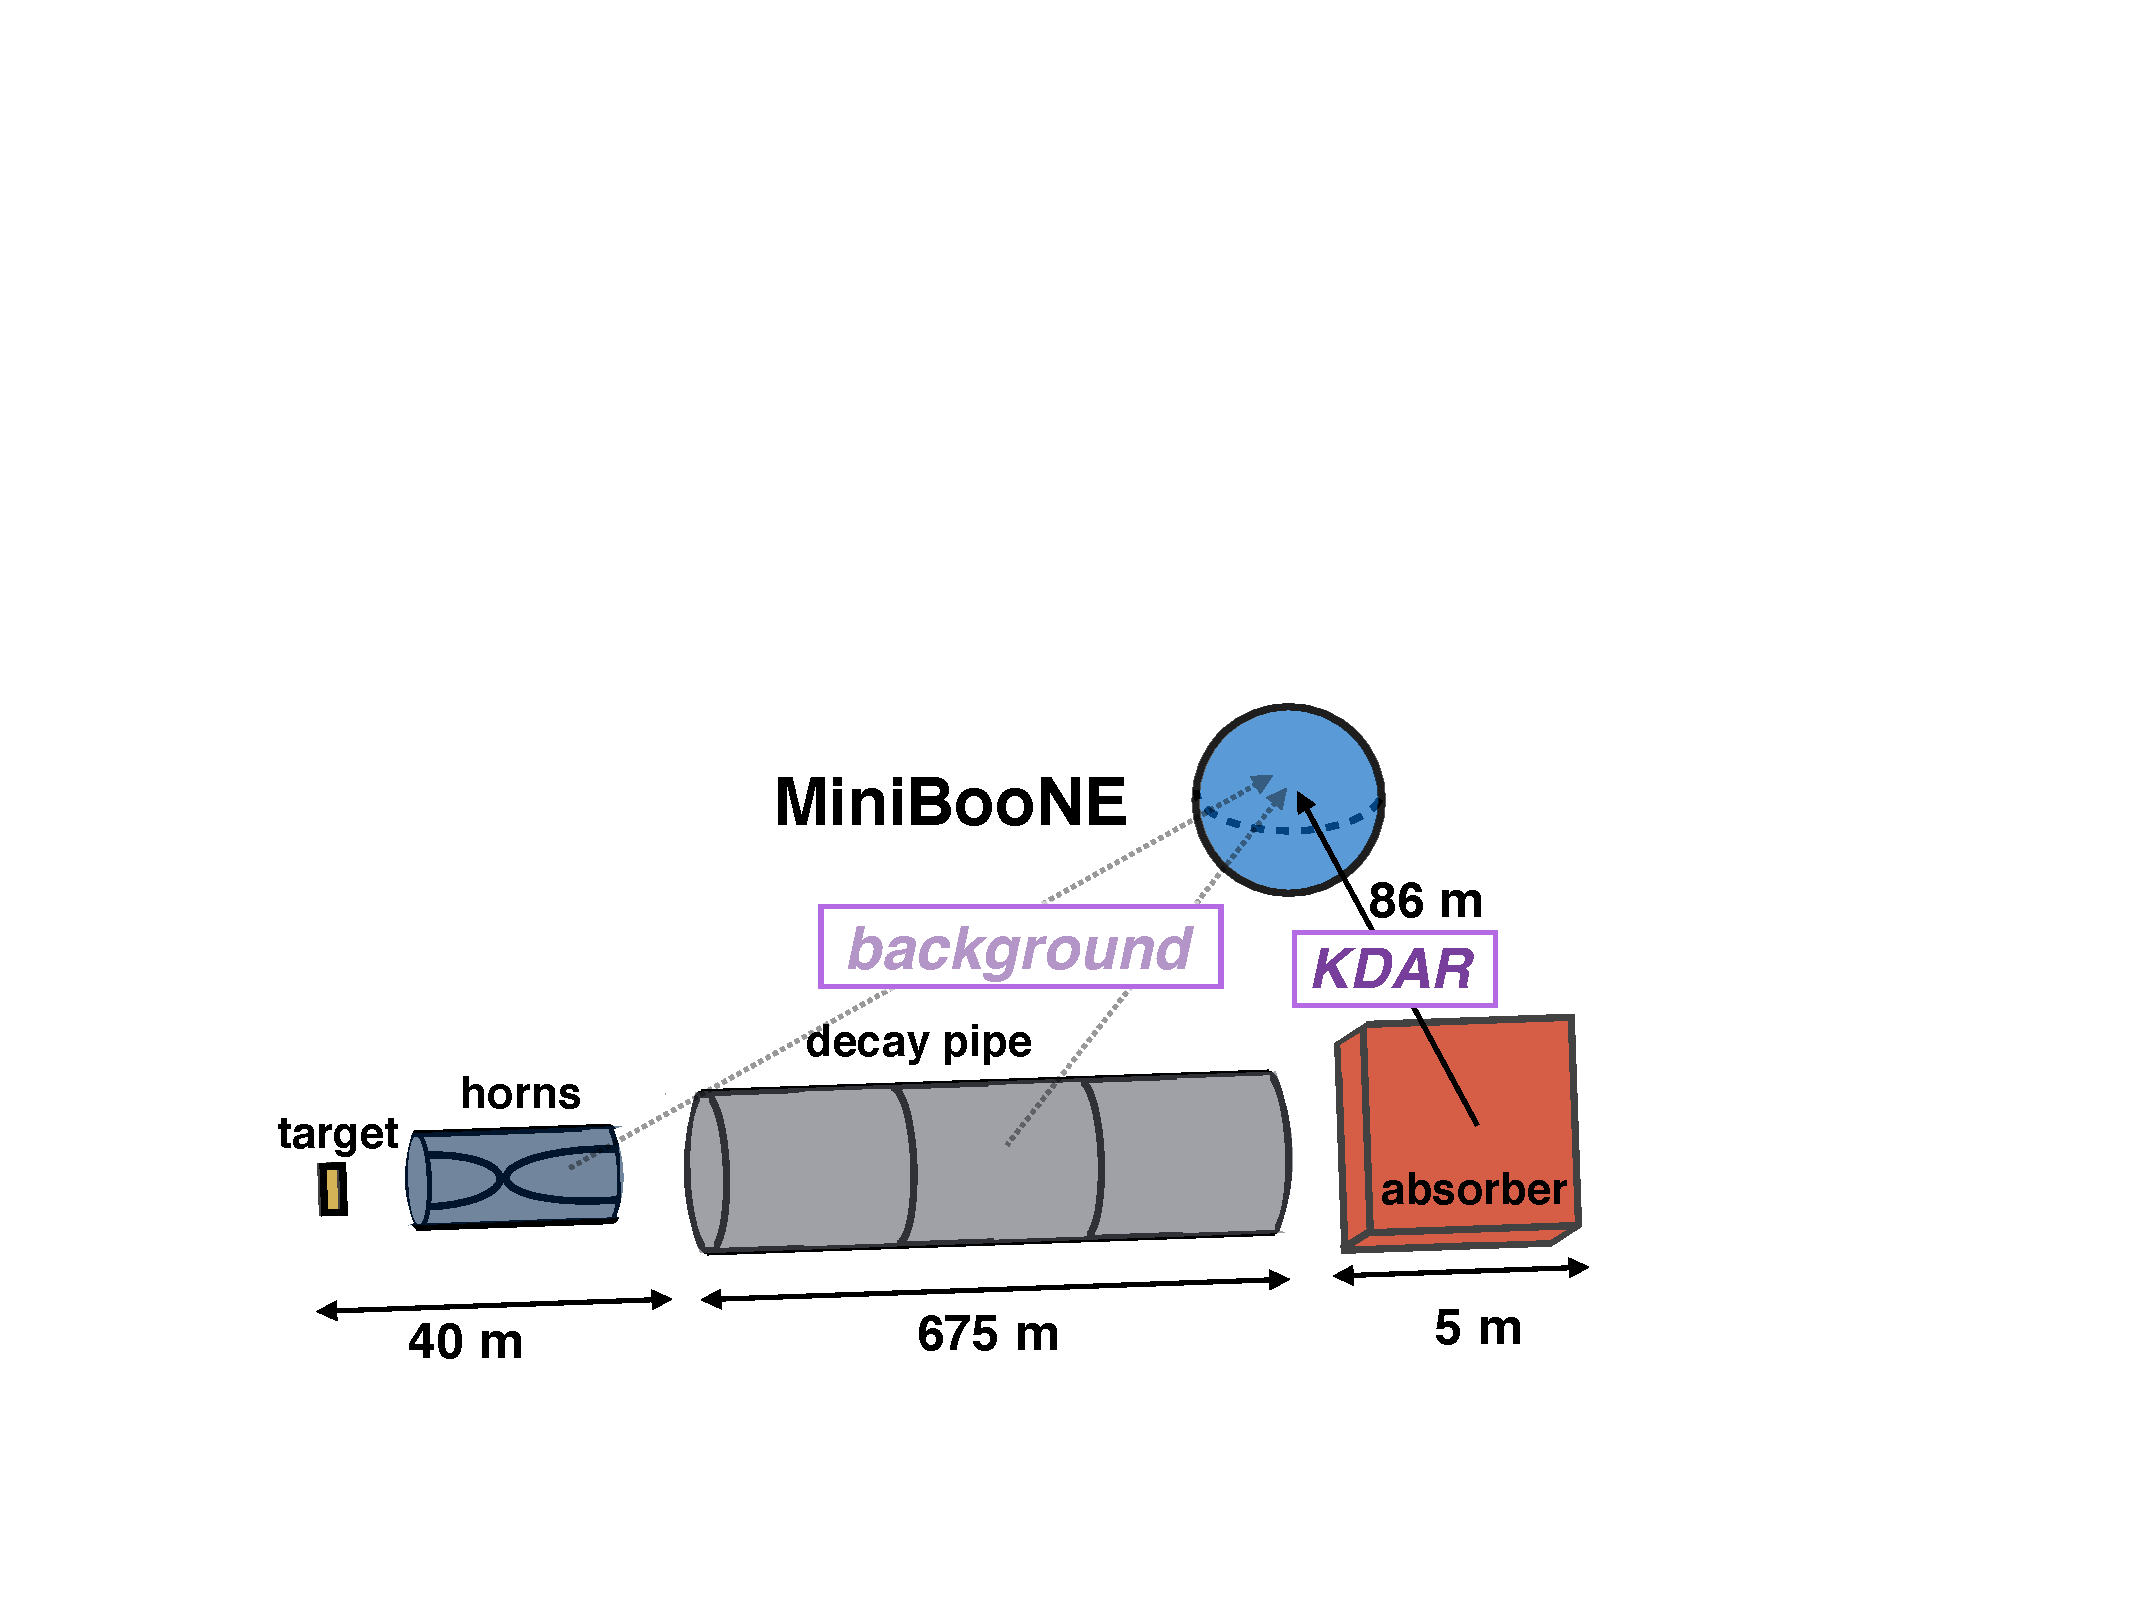
\includegraphics[width=.95\linewidth]{img/beamSchematic} 
%\caption{CAPTION}
%\label{fig:beam}
%\end{figure}


\begin{thebibliography}{7}

\bibitem{chandra}
Chandra, B. \textit{et. al.} (2007). Robust Approach for Estimating Probabilities in Naive-Bayes Classifier. \textit{International Conference on Pattern Recognition and Machine Intelligence}, 11-16.

\bibitem{kwon}
Kwon, N. \textit{et. al.} (2006). Identifying and classifying subjective claims. \textit{Proceedings of the 8th Annual International Digital Government Research Conference}, 76–81.

\bibitem{mccallum}
McCallum, A. \& Nigam, K. (1998). A comparison of event models for naive Bayes text classification. \textit{Proceedings of the 1998 Association for the Advancement of Artificial Intelligence Workshop on Learning for Text Categorization (AAAI’98)}, 41–48.

\bibitem{peters}
Peters, G.,The American Presidency Project [online]. Santa Barbara, CA: University of California (hosted), Gerhard Peters (database). Available from World Wide Web: http://www.presidency.ucsb.edu/

\bibitem{thomas}
Thomas, M. \textit{et. al.} (2006). Get out the vote: Determining support or opposition from Congressional floor-debate transcripts. \textit{Proceedings of the 2006 Conference on Empirical Methods in Natural Language Processing (EMNLP’06)}, 327–335.

\bibitem{xu}
Xu, L. \textit{et. Al.} (2006). Robust Support Vector Machine Training via Convex Outlier Ablation. \textit{Proceedings of the 21st national conference on Artificial intelligence}, Vol 1, 536-542.

\bibitem{yu}
Yu, B. \textit{et. al.} (2008). Classifying party affiliation from political speech. \textit{Journal of Information Technology \& Politics}, 5:1, 33-48, DOI: 10.1080/19331680802149608

\end{thebibliography}

\end{document}
